\section{System Description}
To mitigate some of the issues discussed in Section \ref{problem_analysis}, we propose a new system taking inspiration from the decentralised nature of land-based courier networks. Parcels in transit over land typically pass through several large distribution centres, taking an indirect path to their destination. While this means each individual parcel travels further, it greatly improves the efficiency of the system as a whole. Our system will leverage collaborative autonomy in the form of a fleet of autonomous shuttle ships, which connect a series of `offshore smart ports’ to existing coastal infrastructure.

\begin{figure}[h!]
\begin{center}
\vspace{0.4cm}
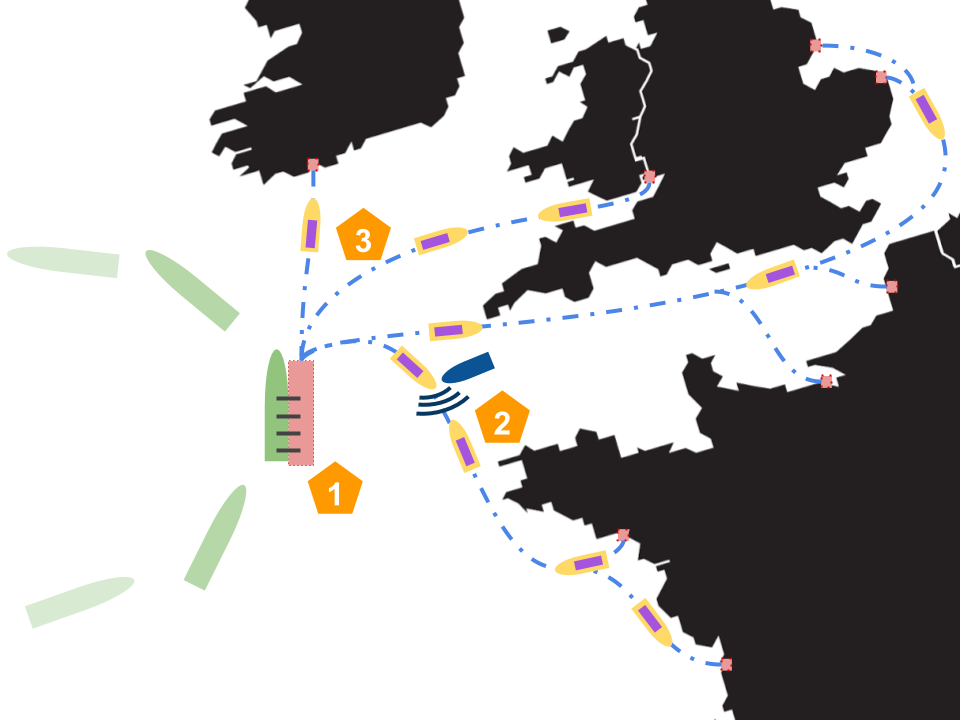
\includegraphics[width=0.7\textwidth]{images/map.png}	
\vspace{0.4cm}
\end{center}
\caption{ A diagram illustrating the main components of our proposed system. \textbf{(1)} An offshore smart port loading and unloading cargo from a docked intercontinental freight ship. \textbf{(2)} An autonomous shuttle ship coordinating with other ships to avoid traffic. \textbf{(3)} An autonomous shuttle ship navigating to a costal port. }
\label{map}	
\end{figure}


Each offshore smart port will act as a regional hub, accepting cargo from existing intercontinental freight ships. This cargo is subsequently forwarded to several coastal ports. The offshore ports are stationary and fixed to the seabed, in much the same way as oil extraction platforms. Aboard each offshore port is an automated container storage and transit system inspired by automated parking facilities \cite{Mathijssen2007}. This system will enable simple storage and retrieval of individual containers through the avoidance of stacking. When each container is ready to leave the offshore port, it is automatically routed to a crane for transfer to a docked vessel. The offshore port will be powered with an onsite nuclear reactor. We assume that it will be both technically feasible and within nuclear regulations to deploy such a reactor to our offshore ports in 2030.

The offshore smart ports will be serviced by a fleet of small autonomous shuttle ships, each capable of transporting a varying number of freight containers between the coastal and offshore ports. The fleet will employ swarm intelligence mechanisms to self-organise. This coordination will help individual ships plan their paths around bad weather and other obstacles, and will also allow the system to respond dynamically to demand at different coastal ports. When goods at a coastal port are ready for dispatch, the shuttle ships will collectively decide an optimal assignment strategy based on their proximity to the collection point. On arrival at the offshore port, the vessel communicates with the storage system to provide information regarding the final destination of the carried goods. Control of the vessel is then delegated to a control system on the offshore port, which is responsible for positioning of the vessel so that the cargo can be offloaded. The shuttle ships will be powered primarily by an on board battery, which is charged at port when necessary. Additionally, on-board solar panels will be used as a means of emergency power generation. We assume that battery technology has developed sufficiently to support the powering of these autonomous vessels for a journey between ports. We also assume that these batteries will be charged using `green’ energy sources.

\begin{figure}[h!]
\begin{center}
\vspace{0.75cm}
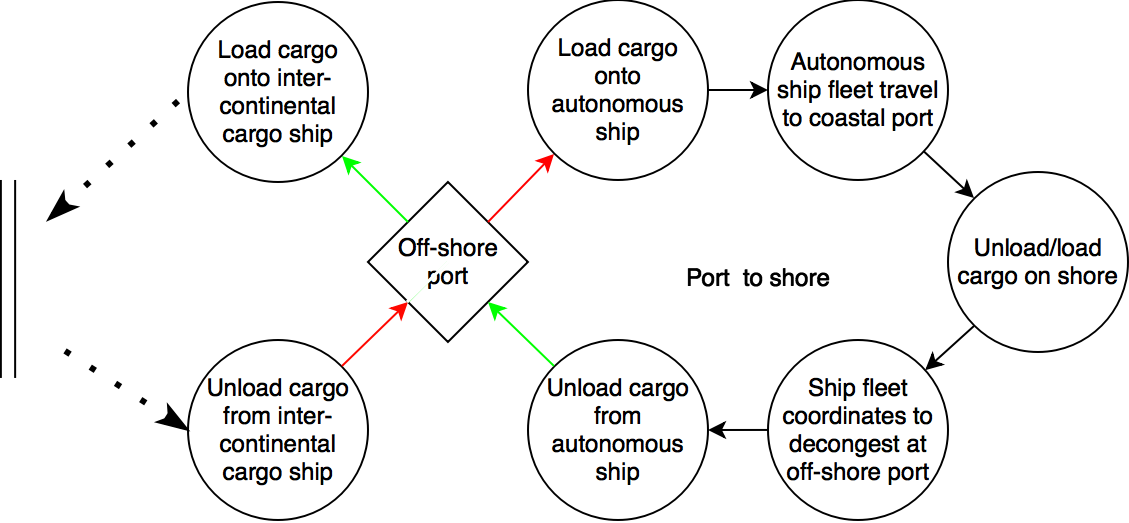
\includegraphics[width=0.9\textwidth]{images/flow.png}	
\end{center}
\caption{A flow chart tracing the flow of cargo through of our system. The left hand side illustrates how cargo enters and leaves the offshore port through intercontinental freight ships. The right-hand side shows how cargo is received from and forwarded by our autonomous shuttle ships. }
\label{flow}	
\end{figure}

Although system components will be fully autonomous, control of the system is transferable to remote human operators in exceptional circumstances, such as malfunction or disaster, in order to mitigate potential adverse consequences of these events. The offshore port and autonomous fleet will initially function at a single location. However we envision that a network of these systems will be deployed at key locations around the world.